\documentclass[12pt,a4paper,oneside]{report}

% ========================================
% Packages
% ========================================
% \usepackage[utf8]{inputenc}
\usepackage[T1]{fontenc}
\usepackage{lmodern}
\usepackage[english]{babel}
\usepackage{CJKutf8}
\usepackage{xcolor}
\usepackage{csquotes}

% Page layout
\usepackage[top=25mm, bottom=20mm, left=20mm, right=20mm]{geometry}

% Graphics and figures
\usepackage{graphicx}
\usepackage{subcaption}
\usepackage{float}

% Mathematics
\usepackage{amsmath,amssymb,amsthm}

% Tables
\usepackage{booktabs}
\usepackage{multirow}

% References and citations
\usepackage[
    backend=biber,
    style=numeric-comp,
    sorting=none,
    date=year,
    maxbibnames=6,
    minbibnames=6,
    giveninits=true,
    doi=true,
    url=true,
    isbn=false,
]{biblatex}
\addbibresource{references.bib}
\DeclareFieldFormat*{title}{\MakeSentenceCase*{#1}}
\DeclareFieldFormat*{titlecase}{\MakeSentenceCase*{#1}}
\DeclareFieldFormat{pages}{#1}
\DeclareFieldFormat{page}{#1}
\DeclareFieldFormat{pagetotal}{#1}
\renewbibmacro{in:}{}
\AtEveryBibitem{\clearlist{language}}

% Line spacing
\usepackage{setspace}
\setstretch{1.3}

% Headers and footers
\usepackage{fancyhdr}
\setlength{\headheight}{16pt}
\pagestyle{fancy}
\fancyhf{}
\fancyhead[R]{\thepage}
\fancyhead[L]{\leftmark}
\renewcommand{\headrulewidth}{0.4pt}
\fancypagestyle{plain}{
  \fancyhf{}
  \fancyhead[R]{\thepage}
  \renewcommand{\headrulewidth}{0pt}
}

% Hyperlinks
\usepackage[colorlinks=true,linkcolor=blue,citecolor=blue,urlcolor=blue]{hyperref}
% \usepackage[hidelinks]{hyperref}

% Theorem environments
\newtheorem{theorem}{Theorem}[chapter]
\newtheorem{lemma}[theorem]{Lemma}
\newtheorem{proposition}[theorem]{Proposition}
\newtheorem{corollary}[theorem]{Corollary}
\theoremstyle{definition}
\newtheorem{definition}[theorem]{Definition}
\newtheorem{example}[theorem]{Example}
\theoremstyle{remark}
\newtheorem{remark}[theorem]{Remark}

% ========================================
% Document Information
% ========================================
\newcommand{\dissertationtitle}{Evolution of Cooperation\\under Environmental Variability}
\newcommand{\authorname}{Masaaki Inaba}
\newcommand{\submissiondate}{March 2026}
\newcommand{\universityname}{University of Tsukuba}
\newcommand{\academicgroup}{Graduate School of Science and Technology}
\newcommand{\degreeprogram}{Degree Programs in Systems and Information Engineering}

% ========================================
% Document Body
% ========================================
\begin{document}

% ========================================
% Cover Page
% ========================================
\begin{titlepage}
    \centering
    \vspace*{5cm}
    {\fontsize{24}{26}\selectfont\bfseries \dissertationtitle\par}
    \vspace*{\fill}
    {\fontsize{20}{22}\selectfont \authorname\par}
    \vspace{1cm}
    {\fontsize{20}{22}\selectfont \submissiondate\par}
    \vspace*{3cm}
\end{titlepage}

% ========================================
% Inside Cover
% ========================================
\newpage
\thispagestyle{empty}
\begin{center}
    \vspace*{5cm}
    {\fontsize{24}{26}\selectfont\bfseries \dissertationtitle\par}
    \vspace*{\fill}
    {\fontsize{20}{22}\selectfont \academicgroup\par}
    {\fontsize{20}{22}\selectfont \degreeprogram\par}
    {\fontsize{20}{22}\selectfont \universityname\par}
    \vspace*{\fill}
    {\fontsize{20}{22}\selectfont \authorname\par}
    \vspace{1cm}
    {\fontsize{20}{22}\selectfont \submissiondate\par}
    \vspace*{3cm}
\end{center}
\newpage

% ========================================
% Abstract
% ========================================
% Front matter: use lowercase roman numerals
\pagenumbering{roman}
\setcounter{page}{1}
\chapter*{Abstract}
\addcontentsline{toc}{chapter}{Abstract}
\input{chapters/0_abstract}

% ========================================
% Table of contents
% ========================================
\tableofcontents
\listoffigures
\listoftables

% ========================================
% Main Content
% ========================================
% Switch to arabic numerals for main matter starting Chapter 1
\clearpage
\pagenumbering{arabic}
\setcounter{page}{1}
\chapter{Introduction}\label{ch:introduction}

Cooperation is fundamental to human society.

\begin{CJK}{UTF8}{min}
{\color{red}
本章は\cite{Inaba2025a,Inaba2025b}および執筆中のChapter3のIntroductionセクションを統合\&拡充して記載する予定です。
現時点 (プレ予備審査時点) では \cite{Inaba2025a}のIntroductionセクションを貼り付けています。
予備審査までにできる限り整えます。
}
\end{CJK}
\vspace*{1cm}

\section{Background}\label{sec:background}

Deepening our understanding of the evolutionary origins of modern human behavior is essential for comprehending the nature of humanity and society.
In anthropology and archaeology, ``modern human behavior" refers to traits unique to or primarily associated with Homo sapiens, marked by abstract thinking, symbolic expression, complex planning, and ultrasociality.
These behaviors include language, religion, mythology, art, music, entertainment, humor, altruism, long-distance trade, and the creation of intergroup networks.
Numerous studies concur that these behavioral patterns emerged during the Middle Stone Age (MSA) in Africa\cite{Mcbrearty2000, Henshilwood2003, dErrico2020, Wilkins2021, Bergstrom2021}.
While there is broad consensus on when and where these behaviors originated, the mechanisms driving their emergence remain enigmatic, despite various proposed theories.

For several years, hypotheses \cite{Potts1996, Potts1998, Potts2013, Potts2018, Potts2020, TrauthMaslin2007, TrauthMaslin2010, TrauthMaslin2014, Ziegler2013, Kalan2020, Siepielski2017, Faith2021} attempting to explain the evolution of hominin behavior by focusing on environmental variability (EV) in Africa during the MSA have garnered significant attention.
Among these, Potts’ variability selection hypothesis (VSH) \cite{Potts1996, Potts1998} proposes that intensified environmental change favored ``versatilists" those capable of rapid adaptation to new environments over ``specialists", who adapt to specific environments, or ``generalists", who adapt across a range of environments.
Here, EV encompasses changes in landscape dynamics (such as land-lake oscillations), climate (such as arid-moist climate oscillations), variations in flora and fauna, ultimately leading to the unpredictability of resource availability.
Initially, this hypothesis was supported by a temporal correlation between intensified environmental changes, the replacement of human species, and the increased complexity of cultural artifacts, such as stone tools and ornaments \cite{Faith2021}.
In addition, the cognitive buffer hypothesis (CBH) \cite{Schuck-Paim2008, Sol2008, Sol2009} provides a neuroscientific basis for VSH, and a mathematical model \cite{Grove2011} demonstrates its theoretical feasibility.
The CBH posits that larger brain sizes in animals, including humans, evolved as a buffer against environmental variability, enhancing survival through improved problem-solving and learning abilities.
In contrast, several theories \cite{Navarrete2011, Will2021, Stibel2023} propose that EV and behavioral diversity do not necessarily drive human encephalization.
These theories emphasize the role of social contexts, as suggested by the social brain hypothesis (SBH) \cite{Whiten1988, Dunbar1998, Barrett2007, Grove2008, Knight2011, Hayes2014, Faith2021, Dunbar2024a}, and consider other factors focus such as dietary influences \cite{DeCasien2017, Grabowski2023}.
The SBH argues that human intellectual abilities evolved in response to the selection pressures of complex social environments, which required the effective management of social relationships within and between groups.
Therefore, much remains unknown about the impact of EV on the evolution of cognitive and behavioral traits in hominins.

Our study suggests that VSH, typically explained through the CBH, may also be connected to the SBH, which is generally considered separate from both VSH and CBH.
While complex social environments encompass various factors, what uniquely characterizes human societies is the extensive and sophisticated cooperation observed, including intergroup cooperation and trade, which contrasts with the intragroup cooperation common in many animal societies.
These advanced social behaviors are central to modern human behavior, and understanding their origins requires focusing on social factors that extend beyond individual-level adaptations, such as those proposed in CBH.
Specifically, we demonstrate that EV fosters intergroup cooperation, which may have contributed to the development of complex social structures.

There are several points of concern when using the term ``group."
First, groups within the complex social environment described by the SBH are nested in a series of fractal-structured networks \cite{Bird2019, Dunbar2020, Dunbar2024a}.
As a result, when smaller groups ally and cooperate to form a larger group, whether this cooperation is viewed as intragroup cooperation within the larger group or intergroup cooperation among the smaller groups depends on the level of analysis.
For simplicity, we assume a certain level of grouping and analyze their intergroup cooperation, though this could alternatively be seen as intragroup cooperation from the perspective of a higher-level group.
Furthermore, while treating groups as units of adaptation is highly debated in evolutionary biology \cite{Smith1976, Okasha2001, Eldakar2011}, our focus here is on cultural evolution rather than biological evolution.
In this cultural context, we assume that a group has a degree of autonomy, treating individual relationships and nested group structures as a black box.
Here, autonomy suggests that the basic behavioral patterns for a group regarding which groups it cooperates with or does not are influenced by intergroup interactions and evolve over time.

In the study of the evolution of cooperation, many studies have been conducted within the framework of evolutionary game theory \cite{Axelrod1981, Nowak2006, Szabo2007, Zaggl2014, Perc2017, West2021}, though most assume a stable environment.
Only a limited number of studies consider environmental factors in the evolution of cooperation, and these, typically in biological or physical contexts, focus on aspects such as extrinsic population variability \cite{Brockhurst2007, Miller2015}, variability in game structure \cite{Gokhale2016, Stojkoski2021}, variability in the strength of selection \cite{Assaf2013}, the impact of EV on learning strategies \cite{Borg2012}, and resource pressure \cite{Pereda2017}.
However, these studies do not fully address our research objective of understanding how EVs influences the evolution of cooperation.

\section{Research Objectives}\label{sec:objectives}

Our research thus investigates how the unpredictability of resource acquisition (EV) may drive the evolution of cooperation among geographically dispersed groups, with a focus on the origins of the social aspects that characterize modern human behavior.

\section{Dissertation Organization}\label{sec:organization}

\textcolor{red}{
ToDo: Describe the structure of the dissertation.
}

\chapter{The base model}\label{ch:2_base_model}

This chapter\protect\footnote{This chapter is based on Inaba and Akiyama (2025) \cite{Inaba2025a}, published in \textit{PLOS Complex Systems}.} introduces a base model to examine our research questions: whether and how environmental variability (EV) promotes the evolution of cooperation.
Although migration is a reasonable response to EV for people during the Middle Stone Age (MSA), we exclude it here to focus on the direct effects of EV on cooperation.
The combined effects of EV and migration are examined in Chapters \ref{ch:3_2Lvl_model} and \ref{ch:4_2D_model}.

\section{Model}\label{sec:2_model}

We use an agent-based simulation model within the framework of evolutionary game theory to investigate how increasing EV influences the evolution of cooperation.
Given the limited availability of detailed data on EV and the spatial distribution of hominid groups during the MSA in Africa, our model adopts a highly abstracted approach, aiming to reveal the general effects of EV based on reasonable assumptions while excluding specific details.
The model operates as follows: several geographically separated regions, each with varying levels of resource accessibility, experience fluctuating resource availability over time (EV).
Each region hosts a single group (agent), and interactions between groups, such as resource exchanges (game) and behavioral pattern transmission (reformation), affect and adjust their relationships.

There are several points of concern when using the term ``group''.
First, groups within the complex social environment described by the social brain hypothesis (SBH) are nested in a series of fractal-structured networks \cite{Bird2019, Dunbar2020, Dunbar2024}.
As a result, when smaller groups ally and cooperate to form a larger group, whether this cooperation is viewed as intragroup cooperation within the larger group or intergroup cooperation among the smaller groups depends on the level of analysis.
For simplicity, we assume a certain level of grouping and analyze their intergroup cooperation, though this could alternatively be seen as intragroup cooperation from the perspective of a higher-level group.
Furthermore, while treating groups as units of adaptation is highly debated in evolutionary biology \cite{Smith1976, Okasha2001, Eldakar2011}, our focus here is on cultural evolution rather than biological evolution.
In this cultural context, we assume that a group has a degree of autonomy, treating individual relationships and nested group structures as a black box.
Here, autonomy suggests that the basic behavioral patterns for a group regarding which groups it cooperates with or does not are influenced by intergroup interactions and evolve over time.

\subsection*{Agent and structure}

In this chapter, each agent represents a single group and has a strategy of either cooperation or defection (``C'' represents a cooperation strategy or a cooperator, while ``D'' represents a defection strategy or a defector).
Initially, all agents are set to D, as intergroup cooperation is considered extremely unlikely \cite{DeDreu2022a, Rodrigues2023}.
This chapter focuses exclusively on intergroup interactions and does not consider intragroup interactions.
While a two-level model would be necessary to analyze the tension between intergroup and intragroup interactions, as seen in multilevel selection studies, a one-level model is suitable here given our focus on intergroup interactions.
All agents are situated within a geographic structure, forming an interaction structure.

The geographic structure is modeled as a line segment with periodic boundary conditions, represented visually as a circle (Fig \ref{fig:model}).
$N$ agents are evenly spaced along the circle.
Although a one-dimensional spatial structure is used for simplicity, more realistic structures can be explored as empirical studies progress.
Migration is not considered in this chapter to keep the model simple as an initial approach.
We incorporate migration in Chapters \ref{ch:3_2Lvl_model} and \ref{ch:4_2D_model}, as it is reasonable to assume that a group might move to a resource-rich region when its resources become scarce.
However, the assumption of no migration is not entirely unrealistic, as some studies have highlighted the tendency for settlement during the MSA \cite{Marean2010, Wadley2011, Kandel2012}.

The interaction structure defines the relationships between agents, which are not limited by the geographic arrangement.
These relationships affect the frequency of games (described later) and are subject to rewiring through reformations (also described later).
The network, where agents are represented as nodes and relationships as edges, is characterized as an undirected, unweighted, and dynamic graph.
The initial network is a regular network with a degree of $k = 4$.

\subsection*{EV}

The resource represents the amount of goods or wealth necessary for survival that a group (agent) can obtain from the natural environment (e.g., food, materials for stone tools required to gather food).
Resources are allocated to each agent at each time step, with the amount varying across different regions.
The node with the highest resource allocation is referred to as the \textit{Source of Resources} (SoR).
The further an agent is located from the SoR geographically, the less resource it receives, as determined by the resource decrement factor, $f_{RD}$.
Specifically, the resource allocated to agent $i$ is calculated as $r_i = r_p - |i - p| f_{RD}$.
Here, $r_i$ represents the resource allocated to agent $i$, $p$ is the index of the SoR, and $|i - p|$ represents the distance between $i$ and $p$, accounting for the boundary conditions, rather than the usual absolute value.
Additionally, there is a universal resource threshold, $\theta$, for all agents; any agent falling below this threshold must reformulate its strategy and relationships.

In this dissertation, EV refers to resource variability, represented by stochastic models.
EV can be divided into variability in distribution of resources among regions and in total quantity of resources across all regions.
Although variations in resource types are also an important consideration, we simplify the model assuming a single resource type.
The two forms of variability are termed regional variability (RV) and universal variability (UV).
RV is a type of EV in which the distribution of resource-rich and resource-poor regions changes over time; specifically, the SoR moves randomly.
The SoR’s index $p_t$ at time $t$ fluctuates according to a stochastic process expressed as $p_{t+1} = ( p_t + \Delta_t ) \mod N$.
Here, $\Delta_t$ is a random integer step uniformly distributed within the range $[ -\sigma_R, \sigma_R ]$, where $0 \leq \sigma_R \leq N / 2$.
UV represents another form of EV in which the total resource quantity fluctuates randomly over time, while the resource distribution between regions remains fixed.
This variability reflects large-scale fluctuations in resource availability across a wide area encompassing all regions.
However, to simplify the implementation, we fix the resource values and instead model UV by varying the threshold value $\theta$, which determines when reformation occurs.
The fluctuation is modeled by a first-order autoregressive process, or AR(1) \cite{Hasselmann1976, Vyushin2012, Salcedo2022}, $\theta_{t+1} = \mu_\theta (1 - \beta) + \theta_t \beta + \epsilon$ with $0 \leq \beta < 1$ and $\epsilon \sim N(0, \sigma_\theta^2)$, where $\mu_\theta$ is the expected value of $\theta$, $\beta$ is the autoregressive coefficient, and $\epsilon$ is a normally distributed noise term with mean $0$ and standard deviation (SD) $\sigma_\theta$.
The intensity of RV is determined by the shift range of the SoR ($\sigma_R$), while the intensity of UV is influenced by the autoregressive coefficient ($\beta$) and the SD of the noise term ($\sigma_\theta$).
We examine the impact of EV on the evolution of cooperation under three scenarios: RV, UV, and combined variability (CV), where both the SoR shifts and the threshold $\theta$ fluctuates.

\begin{figure}[ht]
    \centering
    \includegraphics[width=1.0\linewidth]{figures/2/Fig1.png}
    \caption[Relationships, geographical structure, and EV]{
Relationships, geographical structure, and EV.
Each small circle within the gray circle represents a group (agent, node), with the number inside indicating the resource value.
The gray ring represents the geographical structure, and each line connecting agents denotes a relationship (edge).
(a) In the RV model, the SoR shifts randomly within the geographical structure, and resources are then allocated to other nodes.
Following this, the game and reformation processes occur.
The resource threshold for reformation is fixed at $\theta = 0.5$.
(b) In the UV model, the SoR remains fixed, but the threshold $\theta$ fluctuates randomly, following an AR(1) process.
    }
    \label{fig:model}
\end{figure}

\subsection*{Game}

Communication over resources (such as primitive bartering, giving, looting) between agents is represented by simple pairwise games.
These games can only be played with an opponent who is connected through a network edge.
The probability that agent $i$ selects agent $j$ as its game opponent from its neighbors is $p^G_{i,j} = \frac{1}{n}$;
$n$ is the number of neighbors of $i$, and neighbors refer to agents directly connected to $i$ in the interaction structure network.
The game procedure follows a pairwise public goods game (PGG) \cite{Hardin1968, Binmore1994, Kollock1998, Santos2008} with resource threshold considerations.
First, assume that agent $i$ selects agent $j$.
If the agent is C, it contributes a surplus resource $M_i = \max(r_i - \theta, 0)$.
If the agent is D, it does not contribute any resource.
The contributed resources are multiplied by a factor $b$ ($1 \leq b \leq 2$) and then equally divided between $i$ and $j$.
The payoff table is as follows:
\begin{equation}
\begin{array}{|c|c|c|}
\hline
  & C & D \\
\hline
C & R_i, R_j & S_i, T_j \\
\hline
D & T_i, S_j & P_i, P_j \\
\hline
\end{array}
\end{equation}
\begin{align}
R_i &= \left(\frac{b}{2} - 1\right) M_i + \frac{b}{2} M_j \\
S_i &= \left(\frac{b}{2} - 1\right) M_i \\
T_i &= \frac{b}{2} M_j \\
P_i &= 0
\end{align}

The social optimum, which maximizes the sum of both payoffs, is CC under $b > 1$.
The Nash equilibrium is DD when $b < 2$.
Thus, a social dilemma exists across the defined range of $b$, except at the boundaries.
Additionally, by solving $T_i > R_i > P_i > S_i$, the condition for the game to qualify as a prisoner’s dilemma is $b > 1 + \frac{M_i - M_j}{M_i + M_j}$.
If this condition is not met, then $T_i > P_i > R_i > S_i$.

We have chosen this game model instead of classic pairwise games to implement the condition that only agents with surplus resources can contribute to other agents.
In classic pairwise games, such as the prisoner’s dilemma or the snowdrift game, benefits and costs are fixed at constant values.
This implies that agents would cooperate identically, regardless of resource abundance or scarcity, even under uncertain survival conditions.
This assumption is inconsistent with our research context. Therefore, we have developed and adopted a novel pairwise PGG model that accounts for resource availability.

\subsection*{Reformation}

If, as a result of the games, an agent’s resource falls below the threshold $\theta$, it is considered to have failed to adapt to the environment, triggering a reformation of its strategy and network connections.
An agent $i$ that falls below $\theta$ randomly selects a role model.
The probability that $j$ is chosen as its role model is $p^R_j = \frac{r_j}{\sum_{k \in [1, .., N]} r_k}$.
Agent $i$ imitates $j$’s strategy, with mutation occurring at a probability $\mu$.
Additionally, agents that fall below the threshold disconnect all of their current relationships.
They then randomly select the same number of new neighbors as the number of disconnections and establish new connections.
The probability that agent $j$ is chosen as a new neighbor is proportional to $p^R_j$.
In other words, the higher the resource, the more likely an agent is to be chosen as a role model and a new neighbor.

\subsection*{Evaluation}

The simulation runs for $10,000$ generations, with $100$ independent simulations conducted for each parameter set (Table \ref{tab:2_params}).
Resource allocation and interactions, including games and reformations, occur once per generation.
The proportion of agents employing strategy C in each generation is referred to as the cooperation rate.
The average cooperation rate is calculated as the mean of the cooperation rates across trials, considering only the last $50\%$ of the generations.
To assess the effect of EV on the evolution of cooperation we compared the average cooperation rates across different parameters controlling RV and UV, along with other factors (Table \ref{tab:2_params}).

\begin{table}[ht]
\centering
\caption[Model parameters used in the simulations]{Model parameters used in the simulations.}
\label{tab:2_params}
\begin{tabular}{cp{0.5\textwidth}p{0.3\textwidth}}
\toprule
\textbf{Parameter} & \textbf{Description} & \textbf{Value options} \\
\midrule
$N$ & Number of agents & 100 \\
$\phi_C^0$ & Initial frequency of cooperators & 0 \\
\addlinespace
$k_0$ & Initial degree of the interaction structure network & 4 \\
\addlinespace
$r_{max}$ & Max resource & $1.0$ \\
$f_{RD}$ & Resource decrement factor & $0.02$ \\
\addlinespace
$\sigma_R$ & Shift range of the SoR; controlling the intensity of RV; random shift within $[-\sigma_R, \sigma_R]$ every generation (in Chapters~\ref{ch:3_2Lvl_model} and \ref{ch:4_2D_model}, the intensity of EV is controlled by $p_{EV}$, probability of 1-step shift) & $\{0, 1, \ldots, 49\}$ \\
\addlinespace
$\mu_\theta$ & Expected value of threshold $\theta$ & $0.5$ \\
\addlinespace
$\beta$ & Autoregressive coefficient of the UV; controlling the intensity of UV with $\sigma_\theta$ & $\{0, 0.1, \ldots, 0.9\}$ \\
$\sigma_\theta$ & SD of the noise term of UV; controlling the intensity of UV with $\beta$ & $\{0, 0.1, 0.2\}$ \\
\addlinespace
$b$ & Multiplication factor for PGG & $\{1, 1.1, \ldots, 2\}$ \\
\addlinespace
$\mu$ & Mutation probability in strategy update & $0.01$ \\
\bottomrule
\end{tabular}
\end{table}

\section{Results}\label{sec:2_results}

\subsection*{Effect of RV}

We first examined the impact of RV in isolation, without considering UV.
Specifically, in each generation, the SoR randomly shifts within the range of $[-\sigma_R, \sigma_R]$, accounting for the periodic boundary condition.
The threshold $\theta$, which universally affects the resource welfare of all agents, is fixed at $0.5$.

The results (Fig \ref{Fig:Regional}a) suggest that RV can promote the evolution of cooperation.
To elaborate, when the SoR is fixed ($\sigma_R = 0$), cooperation does not evolve.
As variability slightly increases ($\sigma_R = 1$), the cooperation rate rises to around $10\%$.
For $b \leq 1.7$, further increases in variability do not promote additional cooperation, although the cooperation rate remains higher than when $\sigma_R = 0$ or $1$.
However, for $b \ge 1.8$, greater variability further enhances cooperation.

Despite the overall positive effect of higher variability on cooperation, cooperation is not completely stable and fluctuates with temporary environmental changes.
For example, when $b = 1.8$ and $\sigma_R \in [1, 4, 16]$, the temporal transition (Fig \ref{Fig:Regional}b) shows that the cooperation rate rises and falls dramatically.

\begin{figure}[ht]
    \centering
    \includegraphics[width=0.95\linewidth]{figures/2/Fig2.png}
    \caption[The effect of RV]{
The effect of RV.
(a) The effect of RV across $b \in [1.0, ..., 2.0]$.
The horizontal axis represents the intensity of RV, $\sigma_R$,
and the vertical axis shows the mean cooperation rate over the last $5,000$ generations, averaged across $100$ trials.
(b) Examples of cooperation rate transitions when $b = 1.8$ and $\sigma_R \in [1, 4, 16]$.
The horizontal axis represents generations, and the vertical axis shows the cooperation rate.
Higher RV tends to result in fluctuations of the cooperation rate at higher levels, though convergence is not observed.
    }
    \label{Fig:Regional}
\end{figure}

\subsection*{Effect of UV}

Next, we examined the effects of UV while excluding RV.
As previously defined, UV refers to fluctuations in the threshold $\theta$ across generations, which uniformly affects all agents.
The intensity of this variability is controlled by the autoregressive coefficient $\beta$ and the SD $\sigma_\theta$ of the noise term in the AR(1) stochastic model.
With the SoR fixed at $p = 1$, resources are allocated less as the distance from this node increases.

We found that while UV promotes the evolution of cooperation to some extent, its effect is considerably more limited than that of RV.
For $\sigma_\theta = 0.1$, the cooperation rate gradually increases when $\beta$ exceeds 0.5, but it peaks at just $30\%$ (Fig \ref{Fig:Universal}a).
For $\sigma_\theta = 0.2$, the cooperation rate remains between $20\%$ and $30\%$, regardless of $\beta$, and increasing variability further does not affect these outcomes (Fig \ref{Fig:Universal}a).

\begin{figure}[ht]
    \centering
    \includegraphics[width=0.95\linewidth]{figures/2/Fig3.png}
    \caption[The effect of UV]{
The effect of UV.
(a) The effect of UV across $b \in [1.0, ..., 2.0]$ and $\sigma_\theta \in [0.1, 0.2]$.
The horizontal axis represents the intensity of UV, $\beta$,
and the vertical axis shows the mean cooperation rate over the last $5,000$ generations across $100$ trials.
(The line color scheme of these lines is same as in Fig \ref{Fig:Regional}a.)
(b) Examples of the cooperation rate transition when $b = 1.8$ and $(\beta, \sigma_\theta) \in [(0.1, 0.1), (0.1, 0.2), (0.9, 0.1)]$.
The horizontal axis represents generations, and the vertical axis shows the cooperation rate.
Higher UV tends to result in the cooperation rate fluctuating at higher levels, but convergence is not observed.
    }
    \label{Fig:Universal}
\end{figure}

\subsection*{Effect of CV}

We then examined the combined effects of both RV and UV.
The results (Fig \ref{fig:combination}) show that, consistent with the separate analyses above, RV strongly promotes the evolution of cooperation, while UV has much subtle effect.

\begin{figure}[ht]
    \centering
    \includegraphics[width=0.95\linewidth]{figures/2/Fig4.png}
    \caption[The effect of CV]{
The effect of CV ($b = 1.8$).
(a) and (b) represent cases with $\sigma_\theta = 0.1$, each with a different x-axis.
These plots show that RV increases the cooperation rate significantly, while UV has a limited effect.
(c) and (d) represent cases with $\sigma_\theta = 0.2$, with different x-axis.
The lines are almost flat except in the range $\sigma_R = 0$ to $1$,
indicating that when UV is too high, not only UV but even RV has no effect on the cooperation rate.
    }
    \label{fig:combination}
\end{figure}

\subsection*{Primary drivers of the results}

The results are driven by two key factors:
1. the effects of mutation and EV, which promote fluctuations in cooperation rates, and
2. the coevolution  of cooperation and network structure.

First, RV increases the fluctuations in the cooperation rate, rather than the rate itself.
Fig \ref{fig:mechanism}a shows the effect of EV on strategy distribution in a model that entirely excludes the effects of games and networks.
When these effects are excluded, changes in strategy distribution occur solely due to mutation and strategy updating.
The Y-axis represents the number of agents generated by mutation in one generation, who then serve as role models for strategy updating in the next generation.
These agents are the source of changes in strategy distribution.
The line for RV in the figure shows that as the variability increases, the number of mutated role models increases linearly.
Fig \ref{fig:mechanism}b ``3. (env, C rate)'' shows that the time series of RV and the cooperation rate in each of the 100 trials are completely uncorrelated.
Furthermore, the results remain unchanged even when cross-correlation analysis is performed, accounting for time delays.
Therefore, it is evident that RV does not directly affect the cooperation rate but instead promote fluctuations in it.
This can be explained as follows: agents in poorer regions frequently undergo reformations and mutations.
When RV is small, agents rarely accumulate resources in the next generation, causing them to undergo reformations again.
However, when variability is large, agents may become resource-rich in the next generation, and they potentially survive to influence the strategy updates of other agents.
When RV is large, the cooperation rate is more likely to fluctuate up and down.

\begin{figure}[ht]
    \centering
    \includegraphics[width=1.0\linewidth]{figures/2/Fig5.png}
    \caption[Effects of EV on Cooperation]{
Effects of EV on Cooperation.
(a) The number of mutated role models as a function of RV and UV.
The simulations are based on a model that excludes games.
Therefore, the figure shows how EV and reformation impact the system without the effect of games or network structure.
(b) Correlation analysis through time series ($10,000$ generations) between variables related to EV
(For RV, env refers to the shift distance of the SoR per generation; for UV, env refers to the value of threshold $\theta$),
network structure (degree SD: standard deviation of degrees, hub count: number of nodes with a degree of $10$ or more), and
cooperation (C rate: frequency of C, resource diff: the difference in average resources between C and D, and degree diff: the difference in average degree between C and D).
The mean correlation coefficients are averaged over $100$ trials for both RV and UV.
$b = 1.8$ for all simulations, $\sigma_R = 16$ for RV, and $\beta = 0.7$, $\sigma_{\theta} = 0.1$ for UV.
}
    \label{fig:mechanism}
\end{figure}

Notably, the analytical solution (\ref{eq:n_MR}) aligns closely with the simulation results for RV shown in Fig \ref{fig:mechanism}a.
\begin{align}
E[n_{MR}] &= \sum_{k=0}^n \mu^k (1 - \mu)^{n - k} k \frac{\sigma_R}{N} \notag \\
          &= \frac{n \mu}{N} \sigma_R \label{eq:n_MR}
\end{align}
In this equation, $E[n_{MR}]$ denotes the expected number of mutated role models, which are generated through mutation and later serve as role models for the strategy updates of other agents.
The right-hand side of the equation represents the expected number of mutated agents within a population of reformed agents, $n$, weighted by the effect of RV, $\sigma_R$, across the entire agent population, $N$.
This equation is simplified by applying the formula for the expectation of a binomial distribution.

Second, once the cooperation rate increases, it is likely sustained through the coevolution of cooperation and network structure. Fig \ref{fig:mechanism}b 7 indicates that the cooperation rate is correlated with the difference in resources between C and D. This correlation likely arises because, as the frequency of C increases, mutual support among Cs strengthens, leading to an increase in the average resources of C. Fig \ref{fig:mechanism}b 8 further shows that the difference in resources is strongly correlated with the difference in network degree between C and D. This occurs because, in the reformation process of our model, agents with more resources acquire more edges. Finally, Fig \ref{fig:mechanism}b 6 demonstrates that there is a correlation between the difference in degree and the cooperation rate. This is likely because, as shown in several studies \cite{Santos2005, Santos2006, Santos2008}, heterogeneous degree distributions tend to facilitate cooperation in networks. Thus, a positive feedback loop can form, in which an increase in the cooperation rate induces resource heterogeneity, which subsequently results in network degree heterogeneity, and this network heterogeneity, in turn, reinforces the cooperation rate, which is thought to help sustain the maintenance of a cooperation rate that initially emerged by chance. This explanation is based on correlation and inference, and does not rule out the involvement of other factors. One possible factor is the influence of resource heterogeneity on strategy update frequency, which has been suggested to promote cooperation \cite{Meng2024}. This process may operate alongside the previously described process where an increase in the cooperation rate widens the resource gap between C and D.

In contrast, UV does not significantly promote cooperation for two reasons:
it fails to generate sufficient fluctuation in the cooperation rate, and
it inhibits the coevolution of cooperation and the network structure.
As shown by the two UV lines in Fig \ref{fig:mechanism}a, increasing variability does not substantially increase the number of mutated role models, unlike the linear relationship seen with RV.
Furthermore, when UV is intense and the threshold $\theta$ becomes very large, almost all agents undergo reformation.
This leads to a reduction in network heterogeneity, which is critical for the coevolution of cooperation and network structure.
This is reflected by the strong inverse correlation between UV and network heterogeneity (Fig \ref{fig:mechanism}b 1-2).
The factors that promote cooperation in RV are ineffective in the context of UV, which explains why UV does not significantly promote cooperation.
When RV and UV are combined in the CV model, the results remain consistent, RV promotes cooperation, while UV has a much smaller effect.

In summary, the observed patterns in cooperation rates can be attributed to the combined effects of mutation and EV, as well as the coevolution of cooperation and network structure.
Specifically, when these two factors work well together, as in the RV model, environmental change promotes cooperation.
However, when the first factor is weak and inhibits the second, as in the UV model, cooperation is less likely to evolve.

\section{Summary}\label{sec:2_summary}

This chapter examined the effects of EV on the evolution of intergroup cooperation using a base model without migration.
The results show that RV strongly promotes cooperation, while UV has a weaker effect.
These differences arise from two key factors: the fluctuations in strategy distribution generated by EV, and the coevolution of cooperation and network structure.
Both factors work effectively under RV, whereas under UV, neither factor operates effectively due to insufficient fluctuations and disrupted network heterogeneity.

These findings provide a foundation for examining cooperation under EV.
The next chapter, Chapter \ref{ch:3_2Lvl_model}, extends this base model by incorporating individual-level migration to examine the combined effects of EV and migration.

\chapter{The extended model with migration in hierarchical structure}\label{ch:3_2Lvl_model}

\begin{CJK}{UTF8}{min}
{\color{red}
本章は執筆中です (Modelセクションの完成度: 80\%, Resultsセクションの完成度: 50\%)。
予備審査までにできる限り整えます。
}
\end{CJK}
\vspace*{1cm}

\section{Model}\label{sec_model}

This model is designed to explore the effects of environmental variability and agent mobility on the evolution of cooperation.

\subsection*{Agent, group and structure}\label{sec:structure}

We consider the model composed of multiple regional groups, each inhabited by a number of humans who may migrate between the groups in response to environmental or social pressures.
Within this world, the population is represented by agents and regional groups, and their interaction (see Subsection~\ref{sec:game}) and migration (see Subsection~\ref{sec:migration}) are governed by the geographical and interaction structures (see Figure~\ref{fig:3_model}).

\begin{figure}[htbp]
  \centering
  \includegraphics[width=0.9\textwidth]{figures/3/Model}
  \caption[Illustration of the model structure.]{
Illustration of the model structure.
Regional groups are arranged on a circular geographic structure, where the SoR stochastically moves between groups.
Each group contains agents.
Each group and each agent independently adopt either $C$ (blue) or $D$ (red).
Numbers indicate group resource levels, which decrease with distance from the SoR.
Interaction structures exist at the group level and at the agent level within each group.
  }
  \label{fig:3_model}
\end{figure}

In this model, there are $n_F$ agents and $n_R$ regional groups.
An agent is an abstract representation of the minimal unit of human migration, such as a family.
A group represents the set of agents within a geographically dispersed human habitat.

The geographical structure constrains the positions of groups and the migration of agents.
It is defined as a circular graph, i.e., a ring structure, in which each group is connected to its two neighboring groups.
These connections remain fixed throughout the simulation.
The agents are initially distributed evenly across all groups and can migrate between neighboring groups during the simulation.
The migration results in uneven spatial distributions of agents over time, and some groups can be empty.

The interaction structures constrain the selection of opponents for cooperative or competitive interactions at two levels, i.e., inter-group and intra-group (between agents).
There is a single inter-group interaction structure in the model, while each group has its own intra-group interaction structure and no interactions occur between agents belonging to different groups.
An interaction structure is represented by a weighted, undirected, complete graph whose edge weights are dynamic while its topology remains fixed.
The dynamic edge weight $w_{i,j}$ ($0 \leq w_{i,j} \leq 1$, initialized at $w_0$) denotes the strength of the relationship between nodes $i$ and $j$, where a node represents either a group or an agent, and is proportional to the probability of interaction between them.

Given these structural foundations, the simulation proceeds in four stages: environmental variability, game, migration, and strategy update.
Game and strategy updates occur at both the group and agent levels, in that order.
Each stage is described in the following subsections.

\subsection*{Environmental variability}\label{sec:ev}

The model captures a key feature of the environmental variability observed during the MSA in Africa, namely the unpredictable shifts in the geographical distribution of resources.

To represent this type of variability, we define the source of resources (SoR) as a dynamic point corresponding to the most resource-abundant region.
The SoR moves stochastically across the regional groups introduced in Subsection~\ref{sec:structure} at each simulation time step.
This stochastic movement is formalized as
\begin{equation}
x_{t+1} =
\begin{cases}
\left[ (x_t + \Delta_t - 1) \bmod n_R \right] + 1, & \text{with probability } p_{EV}, \\
x_t, & \text{otherwise},
\end{cases}
\end{equation}
where $x_t$ denotes the index on the circular graph of regional groups indicating the position of the SoR at time $t$, $\Delta_t \in \{-1, +1\}$ is chosen with equal probability, and $p_{EV}$ is a key parameter controlling the intensity of the environmental variability.

The group at which the SoR is located receives a resource value of $1$. The amount of resources allocated to other groups decreases with their distance from the SoR along the geographical structure, reaching $0$ for the group farthest from the SoR.
This resource allocation is formalized as
\begin{equation}
r_i^R = 1 - \frac{d_i}{\left\lfloor \frac{n_R}{2} \right\rfloor}
\end{equation}
where $r_i^R$ denotes the resources received by group $i$, and $d_i$ is the distance between group $i$ and the SoR, calculated with periodic boundary conditions.
The resources of each group are evenly shared among its agents.

\subsection*{Game}\label{sec:game}

Interactions that affect gains and losses of resources, both between groups and between agents, are modeled using a game-theoretic framework.
Because interactions at the group and agent levels often follow the same rules, we occasionally use the term \textit{entity} as a general label for both.
Entity $i$ adopts a strategy $s_i \in \{C, D\}$, where $C$ denotes cooperation and $D$ denotes defection.
The interaction dynamics consist of three sequential phases:
opponent selection,
a pairwise public goods game (PGG), and
an update of the interaction structure.

The opponent selection is based on the relationships between entities specified by the edge weights of the interaction structure.
Each entity $i$ stochastically selects another entity as its opponent, with the probability of selecting entity $j$ given by
\begin{equation}
P(j|i) = \frac{w_{i,j}}{\sum_{k \neq i} w_{i,k}} .
\label{eq:opponent_selection}
\end{equation}

Each selected pair then engages in a pairwise PGG.
Here, we employ a pairwise PGG rather than traditional pairwise games such as the Prisoner’s Dilemma Game and the Stag Hunt Game in order to incorporate both the resource value of each entity and the relationships into the game.
In the game between entity $i$ and $j$, both contribute their respective amounts $c_i$ and $c_j$; the total contribution is multiplied by a constant factor $b$, and the amplified resources are then shared equally between them.
Specifically, $c_i$ is defined as
\begin{equation}
c_i =
\begin{cases}
r_i \times w_{i,j}, & \text{if } s_i = C, \\
0, & \text{if } s_i = D
\end{cases}
\end{equation}
where $r_i$ denotes the resource available to entity $i$ at the time of the game.
In summary, the payoff matrix for entities $i$ and $j$ is
\begin{equation}
\begin{array}{c|cc}
      & C & D \\
\hline
C & \frac{(c_i + c_j) b}{2} - c_i, \frac{(c_i + c_j) b}{2} - c_j & \frac{c_i b}{2} - c_i, \frac{c_j b}{2} \\
D & \frac{c_i b}{2}, \frac{c_j b}{2} - c_j & 0, 0 .
\end{array}
\end{equation}

Finally, the edge weights of the interaction structure are updated to reflect the outcomes of the pairwise games.
Because entities benefit from being connected to $C$ but not to $D$, the direction of change depends on the combination of strategies.
When $C$–$C$, each has an incentive to strengthen the tie, and the relationship becomes stronger.
When $C$–$D$ or $D$–$C$, one side tends to strengthen while the other tends to weaken the tie; these opposing tendencies cancel out, and the relationship remains unchanged.
When $D$–$D$, each has an incentive to weaken the tie, and the relationship becomes weaker.
Formally, the update of the edge weights is given by
\begin{equation}
w_{i,j}' = w_{i,j} + (T - w_{i,j}) \Delta w ,
\end{equation}
where $\Delta w$ ($0 \leq \Delta w \leq 1$) denotes the update rate, and the target value $T$ is set to $1$ if $C$–$C$, $w_{i,j}$ if $C$–$D$ or $D$–$C$, and $0$ if $D$–$D$.

% ここまで修正済み

\subsection*{Migration}\label{sec:migration}

Agents facing resource scarcity stochastically migrate to an adjacent regional group in search of better conditions.
Specifically, the probability that migration occurs is given by $\max \left(1 - \tfrac{r_i^F}{\theta_F}, 0\right) \cdot p_M$, where $r_i^F$ denotes the resource available to agent $i$, $\theta_R$ ($0 < \theta_R < 1$) is the universal threshold shared by all groups, $\theta_F$ is the per-agent threshold obtained by $\theta_F = \tfrac{\theta_R}{n_F / n_R}$, and $p_M$ is a parameter controlling the frequency of migration events.

The migration direction is also probabilistic:
with probability $p_{SoR}$, the agent moves to the neighboring group closer to the SoR;
otherwise, it chooses randomly between the two neighboring groups.

Upon migration, the agent establishes new relationships in the destination group, and discards all previous ones.
Specifically, the edge weights between the agent and the others in the destination group are set to $w_0$, and the edge weights between the agent and the others in the original group are set to $0$.

\subsection*{Strategy update}\label{sec:strategy}

Entities stochastically update their strategies in response to resource scarcity.
Specifically, the probability that an update occurs is given by $\max \left(1 - \tfrac{r_i}{\theta}, 0\right) \cdot p_{SU}$, where $p_{SU}$ is a parameter controlling the frequency of strategy update events.
An entity $i$ that updates its strategy stochastically selects another entity $j$ as its role model, with the probability given by
\begin{equation}
Q(j|i) = \frac{R_j}{\sum_{\substack{k \neq i \\ R_k > \theta}} R_k}
\end{equation}
where $\theta$ denotes the relevant threshold, i.e., $\theta_R$ at the group level and $\theta_F$ at the agent level.
The adopted strategy is then subject to mutation with probability $\mu$, resulting in a stochastic switch between $C$ and $D$.
After the update, all edges of the updated entity are reset to the baseline weight $w_0$.

\subsection*{Evaluation}\label{sec:evaluation}

To examine how environmental variability and agent mobility influence the evolution of cooperation, we conduct simulations across a range of parameter settings, as summarized in Table~\ref{tab:params}.
For each setting, $100$ independent runs of $10000$ generations are carried out. 
As the principal performance indicators, we calculate the cooperation rates $\phi_R^C$ and $\phi_F^C$, defined as the average proportions of groups and agents, respectively, employing strategy $C$ during the last $5000$ generations and averaged over all runs.

\begin{table}[!ht]
\centering
\caption{Model parameters used in the simulations.}
\label{tab:params}
\begin{tabular}{cll}
\hline
\textbf{Parameter} & \textbf{Description} & \textbf{Value options} \\
\hline
$n_R$ & Number of regional groups & $10 \times 2^{\{0, 1, 2, 3\}}$ \\
$n_F$ & Number of agents & $100 \times 2^{\{0, 1, 2, 3, 4, 5, 6\}}$\\
$\phi_C^0$ & Initial frequency of cooperators & $\{0, 0.5, 1\}$ \\
$w_0$ & Initial edge weight & $\{0, 0.1, \ldots, 1.0\}$ \\
$p_{EV}$ & Probability factor for environmental variability & $\{0, 0.1, \ldots, 1.0\}$ \\
$\theta_R$ & Resource threshold at group level & $0.5$ \\
$b$ & PGG multiplier & $\{1.0, 1.1, \ldots, 2.0\}$ \\
$\Delta w$ & Update rate of edge weights & $\{0, 0.1, \ldots, 1.0\}$ \\
$p_M$ & Probability factor for migration events & $\{0, 0.1, \ldots, 1.0\}$ \\
$p_{SoR}$ & Probability of migrating toward SoR & $\{0, 0.1, \ldots, 1.0\}$ \\
$p_{SU}$ & Probability factor for strategy update events & $0.1$ \\
$\mu$ & Mutation probability in strategy update & $\{0, 0.01, 0.05, 0.1\}$ \\
\hline
\end{tabular}
\end{table}

\newpage

\section{Results}\label{sec_results}

\subsection*{Influence of environmental variability and agent mobility}

We conducted computational experiments to investigate how the environmental variability ($p_{EV}$) and the agent mobility ($p_M$) affect the cooperation rates at both the group ($\phi_C^R$) and agent levels ($\phi_C^F$).

Both $\phi_C^R$ and $\phi_C^F$ increase with $p_{EV}$, though with different patterns.
At the group level (Figure~\ref{fig:result1_1}a), $\phi_C^R$ values are around $0.5$ at $p_{EV} = 0$, increase sharply to approximately $0.7$ by $p_{EV} = 0.1$, and then increase gradually to approximately $0.8$ for $p_{EV} > 0.1$.
This pattern does not depend on $p_M$.
At the agent level (Figure~\ref{fig:result1_1}b), $\phi_C^F$ values are below $0.1$ at $p_{EV} = 0$ except at $p_M = 0$;
however, they increase steeply by $p_{EV} = 0.1$ and plateau at levels determined by $p_M$ for $p_{EV} > 0.1$.

While $p_M$ does not affect $\phi_C^R$ (Figure~\ref{fig:result1_1}c), $p_M$ significantly influences $\phi_C^F$ (Figure~\ref{fig:result1_1}d).
When $p_{EV} > 0$, $\phi_C^F$ is approximately $0.6$ at $p_M = 0$, increases to $0.8$--$0.9$ at $p_M = 0.1$, and then decreases linearly for $p_M > 0.1$.
In contrast, when $p_{EV} = 0$, $\phi_C^F$ starts at approximately $0.45$ at $p_M = 0$ and declines rapidly as $p_M$ increases.

\begin{figure}[!ht]
  \centering
  \includegraphics[width=1.0\textwidth]{figures/3/Result1_1}
  \caption[Average cooperation rates as functions of $p_{EV}$ and $p_M$.]{
Average cooperation rates as functions of $p_{EV}$ and $p_M$.
(a) $\phi_C^R$ vs. $p_{EV}$ for different $p_M$ values.
(b) $\phi_C^F$ vs. $p_{EV}$ for different $p_M$ values.
(c) $\phi_C^R$ vs. $p_M$ for different $p_{EV}$ values.
(d) $\phi_C^F$ vs. $p_M$ for different $p_{EV}$ values.
Each data point represents the mean across 100 independent trials, where each trial is averaged over the final 5000 generations.
Other parameters: $n_R = 10$, $n_F = 100$, $\phi_C^0 = 0.5$, $w_0 = 0.3$, $\theta_R = 0.5$, $b = 1.9$, $\Delta w = 0.1$, $p_{SoR} = 0.1$, $\mu = 0.01$.
  }
  \label{fig:result1_1}
\end{figure}

Figure~\ref{fig:result1_2} shows standard deviations corresponding to Figure~\ref{fig:result1_1}.
Although the mean values exhibit clear patterns (Figure~\ref{fig:result1_1}), the high inter-trial variability arises because $\phi_C^R$ and $\phi_C^F$ do not stabilize over time within each individual trial, with different trials converging toward either $0$ or $1$.

\begin{figure}[!ht]
  \centering
  \includegraphics[width=1.0\textwidth]{figures/3/Result1_2}
  \caption{
Standard deviations corresponding to Figure~\ref{fig:result1_1}.
  }
  \label{fig:result1_2}
\end{figure}

To examine the direction of influence between the group-level and agent-level processes, we conducted ablation experiments by selectively disabling specific model components.
The results show that disabling agent-level games, migration, and strategy updates does not significantly affect $\phi_C^R$ values (compare Figure~\ref{fig:result1_1}a,c to Figure~\ref{fig:mechanism1_1}a,c), whereas disabling group-level games and strategy updates markedly suppresses $\phi_C^F$ values (compare Figure~\ref{fig:result1_1}b,d to Figure~\ref{fig:mechanism1_1}b,d).
This asymmetry indicates that group-level processes contribute to agent-level cooperation, while the reverse influence is minimal.

\begin{figure}[!ht]
  \centering
  \includegraphics[width=1.0\textwidth]{figures/3/Mechanism1_1}
  \caption[Ablation experiments corresponding to Figure~\ref{fig:result1_1}.]{
Ablation experiments corresponding to Figure~\ref{fig:result1_1}.
(a) and (c) show $\phi_C^R$ when agent level games, migration, and strategy updates are disabled.
(b) and (d) show $\phi_C^F$ when group level games and strategy updates are disabled.
Comparison with Figure~\ref{fig:result1_1} reveals that $\phi_C^R$ maintains similar patterns regardless of agent level processes, whereas $\phi_C^F$ is substantially reduced without group level processes.
Other conditions are identical to Figure~\ref{fig:result1_1}.
  }
  \label{fig:mechanism1_1}
\end{figure}

The evolution of group-level cooperation by environmental variability can be explained by temporal resource distribution patterns (Figure~\ref{fig:mechanism1_2}).
When $p_{EV} = 0$, the resource-rich region remains fixed at group $1$, creating persistent spatial inequality where groups near SoR remain resource-rich and maintain stable strategies, while distant groups experience resource scarcity and undergo frequent strategy updates (Figure~\ref{fig:mechanism1_2}a).
This spatial segregation prevents the formation of stable cooperative networks across the entire groups.
In contrast, when $p_{EV} > 0$, the location of the resource-rich region shifts over time, ensuring that all regions experience both resource-rich and resource-poor periods.
This temporal equity increases the long-term value of maintaining cooperative relationships through inter-regional games.
As shown in Figure~\ref{fig:mechanism1_2}c, cooperative networks gradually form and stabilize throughout the population.
Groups adopting $C$ strategies build strong reciprocal relationships, while defecting regions become isolated.
These cooperative networks provide resilience against both resource fluctuations and occasional mutations.

\begin{figure}[!ht]
  \centering
  \includegraphics[width=1.0\textwidth]{figures/3/Mechanism1_2}
  \caption[Temporal evolution of group-level cooperation.]{
Temporal evolution of group-level cooperation.
The horizontal axis represents generation, and the vertical axis represents group index.
Blue indicates $C$ and red indicates $D$.
(a) shows the case where $p_{EV} = 0$ with the resource-rich region fixed at group $1$.
(b) shows the case where $p_{EV} = 0.1$ with a shifting resource-rich region.
Occasional mutations introduce $D$, but they quickly revert to $C$.
(c) shows the the transition of the sum of weights between $C$ and $C$.
Other conditions are identical to Figure~\ref{fig:result1_1}.
  }
  \label{fig:mechanism1_2}
\end{figure}

\textcolor{red}{
ToDo: The evolution of agent-level cooperation by environmental variability can be explained by ...
}

\subsection*{Influence of population-related parameters}

Figure~\ref{fig:result2_1} shows the effects of population size parameters $n_R$ and $n_F$ on cooperation rates under different environmental and mobility conditions.

When $p_{EV} = 0.0$ and $p_M = 0.0$, both $n_R$ and $n_F$ have negligible effects on $\phi_C^R$ and $\phi_C^F$ (Figure~\ref{fig:result2_1}a,b).
When $p_{EV} = 0.0$ and $p_M = 0.1$, $\phi_C^R$ remains unaffected by population sizes (Figure~\ref{fig:result2_1}c), whereas $\phi_C^F$ increases with both $n_R$ and $n_F$ (Figure~\ref{fig:result2_1}d).

Under dynamic environmental conditions with $p_{EV} = 0.5$ and $p_M = 0.0$, $\phi_C^R$ decreases slightly with increasing $n_R$ but remains largely unaffected by $n_F$ (Figure~\ref{fig:result2_1}e).
At the agent level, $\phi_C^F$ decreases slightly with increasing $n_R$ but increases slightly with increasing $n_F$ (Figure~\ref{fig:result2_1}f).
These patterns remain essentially unchanged when $p_M$ increases to 0.1 (Figure~\ref{fig:result2_1}g,h).

The initial cooperation rate $\phi_C^0$ influences the evolutionary outcomes (Figure~\ref{fig:result2_2}).
When $\phi_C^0 = 0$, cooperation rates are lower overall compared to $\phi_C^0 = 0.5$ (Figure~\ref{fig:result1_1}), but the qualitative patterns remain unchanged.
In contrast, when $\phi_C^0 = 1$, the patterns change dramatically.
Both $\phi_C^R$ and $\phi_C^F$ approach 1.0 when $p_{EV} = 0$ and decline as $p_{EV}$ increases.
Similarly, both cooperation rates approach 1.0 when $p_M$ ranges from 0 to 0.1 and decline as $p_M$ increases beyond this range.

\subsection*{Influence of network parameters}

The initial network weight $w_0$ influences cooperation evolution at both levels, with smaller values promoting higher cooperation rates (Figure~\ref{fig:result3_1}).
This occurs because $w_0$ determines the interaction strength with newcomers introduced through strategy updates or migration.
When $w_0$ is small, newcomers have weak initial relationships with existing members, limiting their immediate impact on the system.
If a newcomer adopts defection, the low $w_0$ prevents strong interactions that could disrupt established cooperative networks.
In contrast, when $w_0$ is large, defecting newcomers immediately engage in strong interactions with cooperative members, potentially destabilizing the cooperative network and reducing overall cooperation rates.

The relation weight update rate $\Delta w$ positively affects cooperation, with higher values promoting cooperation at both levels (Figure~\ref{fig:result3_2}).
Higher $\Delta w$ values enable relation weights between $C$ pairs to rapidly increase and those between $D$ pairs to quickly decline, thereby accelerating the differentiation between $C$ and $D$ relationships.
This rapid differentiation amplifies the benefits of cooperation and the costs of defection, strengthening selection pressures that favor cooperative strategies.
However, cooperation rates saturate at approximately $\Delta w = 0.3$ as they approach their maximum possible values, beyond which further increases in $\Delta w$ have minimal additional effects.

\subsection*{Influence of other parameters}

We examined the effects of several additional parameters: the SoR orientation ($p_{SoR}$), the PGG multiplier ($b$), and the mutation rate ($\mu$).
The parameter $p_{SoR}$ has no significant effect on cooperation rates.
Higher values of $b$ promote cooperation at both levels, as expected from standard public goods game theory.
Higher $\mu$ values blur the patterns observed in mean cooperation rates while reducing inter-trial variability, but do not alter the qualitative patterns.
Since these results are either trivial or follow directly from model assumptions, detailed results are provided in the Supplementary Material.
\chapter{The 2-dimensional model with migration}\label{ch:4_2D_model}

In Chapters~\ref{ch:2_base_model} and \ref{ch:3_2Lvl_model}, we examined the evolution of cooperation under environmental variability (EV) using models with explicit group structures.
The base model in Chapter~\ref{ch:2_base_model} demonstrated that EV can promote cooperation without migration.
The 2-level model with migration in Chapter~\ref{ch:3_2Lvl_model} extended this by introducing individual-level migration and demonstrated that EV can still promote cooperation.
Moreover, moderate migration promotes cooperation while excessive migration hinders it.
However, the 2-level model is relatively unique and limits clear comparison with existing studies on cooperation and migration.
In this chapter\protect\footnote{This chapter is based on Inaba and Akiyama (2025) \cite{Inaba2025b}, published in \textit{Chaos, Solitons \& Fractals}.}, we adopt a 2-dimensional (2D) space, which is widely used in the literature, diverging from the group-structured frameworks of Chapters \ref{ch:2_base_model} and \ref{ch:3_2Lvl_model} to prioritize comparability with prior works.

The evolution of cooperation among mobile agents has been studied actively.
Dugatkin and Wilson (1991) \cite{Dugatkin1991} performed pioneering work in this area, demonstrating that the effectiveness of Axelrod's Tit-for-Tat strategy \cite{Axelrod1981} can be undermined by mobile defectors (Rover strategy) when migration costs are low, although their model employed a patch structure rather than a 2D space.
More contemporary research in 2D spatial settings, where both cooperators and defectors can migrate, was initiated by Vainstein and Arenzon (2001) \cite{Vainstein2001} and established by Vainstein et al. (2007) \cite{Vainstein2007}.
They demonstrated that mobility can have contrasting effects: under certain conditions, it promotes cooperation by facilitating cooperator clustering and separation from defectors, while under other conditions, it hinders cooperation by generating strategic chaos.
These developments are reviewed in Perc and Szolnoki (2010) \cite{Perc2010}.
Building on Vainstein's framework, various migration strategies \cite{Cong2012, Chen2012, He2020, Dhakal2020, Ren2021, Yang2023, Zhang2025} differing in trigger conditions and migration distance have been proposed more recently.
However, to the best of our knowledge, no study has examined the effects of extrinsic EV on the evolution of cooperation among mobile agents.

This chapter addresses this gap within Vainstein's framework by modeling EV as randomly moving resource-rich spots (Sources of Resources; SoRs) across a 2D space and agent mobility as resource-seeking migration.
Through extensive simulations, we examine whether and how these factors jointly promote cooperation.

\section{Model}\label{sec:4_model}

In this chapter, we developed a multiagent simulation model to examine how agent mobility and EV jointly influence the evolution of cooperation in spatially structured populations.
Due to the limited availability of archaeological data on spatial resource distributions and hominin behavioral patterns during the MSA, we adopted an abstracted approach that prioritizes the identification of fundamental mechanisms over reproducing specific historical scenarios.
This model incorporates four key processes, i.e.,
(i) EV on a 2D lattice,
(ii) pairwise game interactions,
(iii) conditional agent migration driven by resource availability, and
(iv) strategy updating.
These processes are described in the following subsections.

\subsection*{Environmental variability}

The spatial structure is represented by a 2D lattice with periodic boundary conditions.
Here, $N$ agents are distributed randomly across the cells, and each cell contains at most one agent.
Each cell maintains a resource level that varies both spatially and temporally.
We define a Source of Resources (SoR) as a focal point that generates spatial resource gradients in the environment, and these SoRs serve as simplified representations of the natural foraging areas commonly found near rivers, lakes, and coastlines.
Each SoR creates a gradient where resource availability typically decreases with increasing distance from the SoR.
In addition, multiple SoRs may coexist, thereby forming overlapping zones of resource abundance.

In this model, each agent accumulates resources (represented by the agent's fitness value) through interactions, and local prosperity is defined by a resource threshold $\theta_{x,y}$ for each cell $(x, y)$, where $0 \leq \theta_{x,y} \leq 1$.
Agents with fitness values that are less than the threshold $\theta_{x,y}$ are more likely to migrate and update their strategies, and agents with fitness values greater than the threshold remain unchanged.
Therefore, locations with lower thresholds impose less pressure for behavioral change, indicating that these locations are prosperous and rich in resources.
Here, the threshold $\theta_{x,y}$ is determined by the cumulative influence of all SoRs and is calculated as follows:
\begin{equation}
\theta_{x,y} = \frac{D_{x,y} - D_{\min}}{D_{\max} - D_{\min}}, \quad D_{x,y} = \sum_{i=1}^{n_{SoR}} d_{x,y}^{(i)}
\end{equation}
where $n_{SoR}$ denotes the number of SoRs, $d_{x,y}^{(i)}$ denotes the Euclidean distance from cell $(x, y)$ to the $i$-th SoR, calculated under periodic boundary conditions, and $D_{\min}$ and $D_{\max}$ denote the minimum and maximum values of $D_{x,y}$ across the entire grid, respectively.

We examine two spatial configurations, which we refer to as 1-SoR and 2-SoR.
In the 1-SoR configuration (a $200\times200$ grid), a single SoR generates a concentric resource gradient, capturing the essential geographical pattern of an oasis-like environment (Figure~\ref{fig:ev}a).
In the 2-SoR configuration (a $400\times200$ grid), two SoRs generate a corridor of resource gradient, capturing the essential geographical pattern of riverine or coastal environments where resources are distributed along a line (Figure~\ref{fig:ev}b).

\begin{figure}[!ht]
\centering
\includegraphics[width=1.0\linewidth]{figures/4/Fig1.png}
\caption[Spatially heterogeneous prosperity patterns generated by SoR(s)]{
Spatially heterogeneous prosperity patterns generated by SoR(s).
The colors indicate the resource threshold $\theta_{x,y}$.
(a) A single SoR located at $(100, 100)$ on a $200\times200$ grid generates a concentric resource gradient.
(b) Two SoRs located at $(100, 100)$ and $(300, 100)$ on a $400\times200$ grid generate a band-shaped resource gradient.
(c) and (d) Examples of the stochastic movement of SoRs that dynamically reshapes the resource landscapes.
}\label{fig:ev}
\end{figure}

EV is modeled through the stochastic movement of SoRs, reflecting the unpredictable nature of the landscape dynamics observed during the MSA in Africa.
Each SoR moves to a randomly selected adjacent cell within the Moore neighborhood with a probability $p_{EV} \, (0 \leq p_{EV} \leq 1)$ at each time step, and the direction is selected uniformly at random from the eight neighboring cells.
In this process, the parameter $p_{EV}$ governs the intensity of the EV, where $p_{EV} = 0$ corresponds to a static environment, and higher $p_{EV}$ values represent more intense EV.

Throughout this chapter, the neighborhood is defined as the Moore neighborhood (i.e., eight neighboring cells).
This choice better approximates the continuous spatial movement of SoRs and mobile agents than the von Neumann neighborhood (i.e., four orthogonal cells), where movement is restricted to only cardinal directions.
In addition, for distance calculations, particularly when determining resource gradients from SoRs, the Euclidean distance is employed to produce smooth, circular gradients that better represent natural resource distributions than other metrics, e.g., the Manhattan or Chebyshev distances.

\subsection*{Game}

Games represent cooperative or competitive interactions between agents that involve the gain or loss of resources.
Each agent holds a strategy, either cooperation ($C$) or defection ($D$), which determines its behavior in interactions.
In every time step, each agent plays pairwise games with all its neighbors and accumulates a payoff $\pi_j$, which is then converted into fitness $\omega_j$ ($j \in [1,\ldots,N]$, $0 < \omega_j < 1$), representing the agent's resource level.

The payoff matrix of the game is defined as follows:
\begin{equation}
\begin{array}{c|cc}
  & C & D \\
\hline
C & R & S \\
D & T & P
\end{array}
\end{equation}
where $R = 1$, $0 < T < 2$, $-1 < S < 1$, and $P = 0$.
To ensure the robustness of the results across a range of social dilemma contexts, we consider various game structures, including the Prisoner's Dilemma ($T > R > P > S$), Stag Hunt ($R > T > P > S$), and Snowdrift ($T > R > S > P$) games.

The accumulated payoff $\pi_j$ is transformed into the fitness $\omega_j$ using a sigmoid function as follows:
\begin{equation}
\omega_j = \frac{1}{1 + \exp(-k(\pi_j - \pi_0))}
\end{equation}
where $k$ determines the steepness of the sigmoid curve, and $\pi_0$ sets the baseline payoff at which $\omega_j = 0.5$.
Here, we set $k = 1$ for moderate sensitivity and set $\pi_0 = 4.0$ to center the sigmoid around common payoff values found in mixed-strategy populations.
Given that each agent can accumulate payoffs from up to eight of its neighbors, the theoretical payoff range is $8S$ to $8R$ and $8P$ to $8T$ for cooperators and defectors, respectively.
With our parameter constraints, this yields a payoff range of $-8 < \pi_j < 16$.

\subsection*{Migration}

At each time step, agents migrate if their fitness $\omega_j$ is less than the resource threshold $\theta_{x,y}$ at their current location.
Any agent that meets this condition migrates with probability $p_M$ and remains at the location with the complementary probability $1 - p_M$.
The migration direction follows a resource-oriented bias, where an agent moves toward a neighboring cell with the lowest $\theta_{x,y}$ value with probability $p_{SoR}$ (SoR orientation) and moves randomly within the neighborhood with the complementary probability $1 - p_{SoR}$.
Cells occupied by other agents are excluded from the candidate destinations.
The agents migrate asynchronously in a randomized order to avoid movement conflicts.

\subsection*{Strategy update}

At each time step, agents update their strategies synchronously if their fitness $\omega_j$ is less than the resource threshold $\theta_{x,y}$.
Any agent that meets this condition adopts the strategy of the most successful neighbor (i.e., the neighbor with the highest fitness).
This process is subject to mutation, where the adopted strategy is replaced by the opposite strategy (e.g., from $C$ to $D$ or vice versa) with probability $\mu$.

We note that asynchronous updating \cite{Huberman1993, Zhang2025a} is more realistic and the choice of updating protocol can significantly affect outcomes in densely packed models \cite{Huberman1993}.
However, unlike densely connected lattice models where agents interact with many neighbors simultaneously, our agents typically interact with only a few neighbors on each resource patch.
This sparsity reduces the interdependence between neighboring strategy updates, making the dynamics largely insensitive to the updating protocol.

\subsection*{Evaluation}

To investigate the effects of EV and agent mobility on the evolution of cooperation, simulations are performed under a range of parameter configurations, as shown in Table~\ref{tab:4_params}.

Each configuration is evaluated through $100$ independent trials of $10000$ generations each.
As the primary outcome measure, we compute the cooperation rate $\phi_C$, which is defined as the average proportion of agents employing the $C$ strategy at the end of each generation (following the strategy update process), averaged over both the final $5000$ generations and all $100$ independent trials.

\begin{table}[!ht]
\centering
\caption[Model parameters used in the simulations]{Model parameters used in the simulations.}
\label{tab:4_params}
\begin{tabular}{cp{0.6\textwidth}p{0.2\textwidth}}
\toprule
\textbf{Parameter} & \textbf{Description} & \textbf{Value options} \\
\midrule
$W \times H$ & Grid dimensions & $200 \times 200, 400 \times 200$ \\
$N$ & Number of agents & $\{500, 1000, 2000,$ $4000, 8000, 16000\}$ \\
$\phi_C^0$ & Initial frequency of cooperators & $\{0, 0.5, 1\}$ \\
\addlinespace
$n_{SoR}$ & Total number of SoRs & $\{1, 2\}$ \\
\addlinespace
$p_{EV}$ & Probability of SoR shift; controlling the intensity of EV (shift range of the SoR, $\sigma_R$, in Chapter~\ref{ch:2_base_model}) & $\{0, 0.1, \ldots, 1\}$ \\
\addlinespace
$R$ & Payoff for mutual cooperation & $1$ \\
$T$ & Payoff for defection against cooperator & $\{0, 0.1, \ldots, 2\}$ \\
$P$ & Payoff for mutual defection & $0$ \\
$S$ & Payoff for cooperation against defector & $\{-1, -0.9, \ldots, 1\}$ \\
\addlinespace
$p_M$ & Direct probability of migration for agents below threshold (multiplied by resource deficit in Chapter~\ref{ch:3_2Lvl_model}) & $\{0, 0.1, \ldots, 1\}$ \\
\addlinespace
$p_{SoR}$ & Probability of migrating toward SoR & $\{0, 0.1, \ldots, 1\}$ \\
\addlinespace
$\mu$ & Mutation probability in strategy update & $\{0, 0.01\}$ \\
\bottomrule
\end{tabular}
\end{table}

\section{Results}\label{sec:4_results}

\subsection*{Influence of environmental variability and agent mobility}\label{sec:4_key_results}

Figure~\ref{fig:4_key_result} shows the combined effects of EV ($p_{EV}$) and agent mobility ($p_M$) on the cooperation rate $\phi_C$.
As can be seen, in stable environments ($p_{EV} = 0$) or with low agent mobility ($p_M \lesssim 0.2$), cooperation fails to evolve.
In contrast, with sufficient agent mobility ($p_M \gtrsim 0.2$), even modest EV ($p_{EV} = 0.1$) promotes cooperation; however, further variability ($p_{EV} > 0.1$) does not enhance cooperation.
In addition, agent mobility promotes cooperation with any level of EV ($p_{EV} > 0$).

\begin{figure}[!ht]
\centering
\includegraphics[width=0.7\linewidth]{figures/4/Fig2.png}
\caption[Influence of environmental variability ($p_{EV}$) and agent mobility ($p_M$) on the cooperation rate ($\phi_C$)]{
Influence of EV ($p_{EV}$) and agent mobility ($p_M$) on the cooperation rate ($\phi_C$).
The figure shows that cooperation emerges only when both $p_{EV} \gtrsim 0.1$ and $p_M \gtrsim 0.2$, with neither factor alone being sufficient to promote cooperation.
Each cell shows the mean value over 100 independent runs.
The results are shown for a representative parameter set ($N = 1000$, $\phi_C^0 = 0.0$, 2-SoR, $T = 1.2$, $S = -0.2$, $p_{SoR} = 0.1$, $\mu = 0.01$).
Qualitatively similar patterns are observed for other parameter configurations.
The standard deviations across runs are less than $0.15$ for all cells.
}\label{fig:4_key_result}
\end{figure}

Figure~\ref{fig:4_temporal_01_10} shows the role of EV in the evolution of cooperation.
This representative simulation is presented to understand the temporal dynamics underlying the statistical patterns displayed in Figure~\ref{fig:4_key_result}.
Whereas Figure~\ref{fig:4_key_result} considers fixed variability levels throughout the simulation, here we apply a cyclic $p_{EV}$ alternating between stable and variable conditions every $2000$ generations over a total of $10000$ generations.
Under these cyclic conditions, cooperation initially increases to slightly less than $50\%$ during the first stable phase and then plateaus, as shown in Figure~\ref{fig:4_temporal_01_10}a.
A pronounced increase is observed once the system enters the variable phase, which reinforces the conclusion that EV plays a pivotal role in promoting cooperation.

\begin{figure}[!ht]
\centering
\includegraphics[width=1.0\linewidth]{figures/4/Fig3.png}
\caption[Temporal dynamics under cyclic environmental variability]{
Temporal dynamics under cyclic EV.
The figure demonstrates that EV drives cooperation by disrupting stable defector groups in resource-rich areas and facilitating the formation of multiple small cooperator groups.
(a) Cooperation rate over $10000$ generations with $p_{EV}$ alternating between stable ($p_{EV} = 0$) and variable ($p_{EV} = 0.1$) phases every $2000$ generations.
(b)--(f) Spatial snapshots at each generation.
Blue and red dots represent cooperators and defectors, respectively.
Background colors indicate the resource threshold $\theta_{x,y}$ as in Figure~\ref{fig:ev}.
Parameter settings: $N = 1000$, $\phi_C^0 = 0.0$, 2-SoR, $T = 1.2$, $S = -0.2$, $p_M = 1.0$, $p_{SoR} = 0.1$, $\mu = 0.01$.
}\label{fig:4_temporal_01_10}
\end{figure}

The observed dynamics can be understood as a three-stage process:
(i) the formation of a few large defector groups fixed in resource-rich areas,
(ii) their collapse induced by EV, and
(iii) subsequent emergence of several small cooperator groups.
Figures~\ref{fig:4_temporal_01_10}b--f show snapshots from the simulation presented in Figure~\ref{fig:4_temporal_01_10}a.
A full video showing this process is provided in the \nameref{appendix}.
In the first stable phase as shown in Figure~\ref{fig:4_temporal_01_10}b, the agents in prosperous areas have no need to cooperate or move, whereas those in less prosperous areas must cooperate or move to prosperous areas.
At the boundaries between these two areas, fixed walls are formed by defectors who do not need to change their strategies or move further.
During the next variable phase as shown in Figures~\ref{fig:4_temporal_01_10}c--e, agents located on boundaries are forced to cooperate or move due to the environmental changes, thereby leading to the collapse of the stable defector group as shown in the central area of Figure~\ref{fig:4_temporal_01_10}c.
In place of the defector group, the agents form several small cooperator groups to survive even in severe environmental conditions (Figure~\ref{fig:4_temporal_01_10}d).
Then, the same process occurs in the areas at both ends of the figure (Figures~\ref{fig:4_temporal_01_10}e and f).

In contrast, cooperation cannot evolve if the agent mobility is insufficient relative to the intensity of the EV (refer to the lower area of Figure~\ref{fig:4_key_result}),
which occurs because excessively rapid SoR movement prevents the formation of both defector structures and small cooperator groups, as shown in Figure~\ref{fig:4_temporal_01_01}.
Thus, EV and sufficient agent mobility promote cooperation by preventing fixed defector structures and encouraging the agents to form cooperator groups for survival.

\begin{figure}[!ht]
\centering
\includegraphics[width=1.0\linewidth]{figures/4/Fig4.png}
\caption[Temporal dynamics under cyclic environmental variability with low agent mobility]{
Temporal dynamics under cyclic EV with low agent mobility.
In contrast to Figure~\ref{fig:4_temporal_01_10} ($p_M = 1.0$), here lower mobility ($p_M = 0.1$) prevents agents from keeping up with the EV.
As a result, cooperation fails to evolve.
All other parameters and the interpretation of the visual elements are the same as in Figure~\ref{fig:4_temporal_01_10}.
}\label{fig:4_temporal_01_01}
\end{figure}

\subsection*{Influence of other parameters on cooperation rate}

To gain further insights into the findings presented above and assess their robustness, we investigated the effects of additional parameters, including the population size ($N$), the number of SoRs ($n_{SoR}$), the initial frequency of cooperators ($\phi_C^0$), the SoR orientation ($p_{SoR}$), the payoff parameters ($T$, $S$), and the mutation rate ($\mu$).

\subsubsection*{Population size}

Larger population size promotes cooperation to some extent, as shown in Figure~\ref{fig:4_population}, because the cooperators can more easily find other cooperators when the population size is sufficiently large.

Another notable observation is that the cooperation rates for $(p_{EV}, p_M) = (0.0, 0.1)$ (red dashed line) and $(0.1, 0.1)$ (blue dashed line) exhibit a crossover at approximately $N = 2000$.
For small populations ($N < 2000$) with low agent mobility, cooperation evolves more readily without EV.
In stable environments ($(p_{EV}, p_M) = (0.0, 0.1)$), both the defector and cooperator groups persist once established, although the formation of these groups is slow due to the low agent mobility.
In contrast, EV with low agent mobility ($(p_{EV}, p_M) = (0.1, 0.1)$) creates perpetual fluidity that prevents the formation of both structures.

Larger populations alter this relationship.
Larger populations increase the encounter rate among cooperators, which allows for the formation of cooperator groups even under EV.
In stable environments, the structures remain fixed, thereby limiting the impact of the higher encounter rate.
In contrast, the higher encounter rate in fluid environments facilitates group formation.
Thus, EV becomes advantageous for cooperation above the critical population size.

A less prominent but similar crossover occurs at approximately $N = 8000$ between $(p_{EV}, p_M) = (0.0, 0.1)$ (red dashed line) and $(p_{EV}, p_M) = (0.0, 1.0)$ (red solid line).
This crossover reflects the spatial constraints of the defector groups in stable environments ($p_{EV} = 0$).
For $N \lesssim 8000$, high mobility ($p_M = 1.0$) allows more agents to reach the resource-rich areas where cooperation is not required.
In contrast, low mobility ($p_M = 0.1$) keeps the agents in peripheral areas where cooperation is required for survival.

However, larger populations ($N \gtrsim 8000$) exhibit three nested zones:
central rich areas, where cooperation is not required;
surrounding moderate areas, where the agents can survive through cooperation; and
the most peripheral harsh areas, where agents cannot survive even with cooperation because the resource threshold exceeds what can be provided through cooperation.
Under these conditions, high mobility allows the agents to escape from the harsh areas to the moderate cooperative areas, whereas low mobility traps the agents in the harsh areas.
In addition, the central rich areas have already reached their physical capacity due to the large population;
thus, further population increases have no effect in these areas.
Consequently, the effect of mobility on the cooperation rate ($\phi_C$) reverses as the population size increases.

\begin{figure}[!ht]
\centering
\includegraphics[width=0.7\linewidth]{figures/4/Fig5.png}
\caption[Influence of population size ($N$) on cooperation rate ($\phi_C$)]{
Influence of population size ($N$) on cooperation rate ($\phi_C$).
The figure shows two crossovers: at $N \approx 2000$ between $(p_{EV}, p_M) = (0.0, 0.1)$ (red dashed) and $(0.1, 0.1)$ (blue dashed), and at $N \approx 8000$ between $(0.0, 0.1)$ (red dashed) and $(0.0, 1.0)$ (red solid).
These crossovers reflect how population size alters the relative benefits of EV and mobility through changes in cooperator encounter rates and spatial resource distribution.
Parameter settings: $\phi_C^0 = 0.0$, 2-SoR, $T = 1.2$, $S = -0.2$, $p_{SoR} = 0.1$, $\mu = 0.01$.
The results for $N = 32000$ are omitted because they exhibited negligible differences from $N = 16000$.
}\label{fig:4_population}
\end{figure}

\subsubsection*{Number of SoRs and initial cooperation rate}

Both the number of SoRs ($n_{SoR}$) and the initial frequency of cooperators ($\phi_C^0$) have a significant influence on the results.
While the 2-SoR configuration forms large band-shaped defector groups (Figure~\ref{fig:4_temporal_01_10}b), the 1-SoR configuration only forms a small, circular resource-rich area (Figure~\ref{fig:4_1sor}b).
When a large defector group collapses and is replaced by small cooperator groups, as observed with the 2-SoR setting, the impact on the overall system is substantial.
In contrast, under the 1-SoR setting, when a small defector group undergoes the same replacement, the effect is less conspicuous than in the 2-SoR setting (Figure~\ref{fig:4_1sor}a).
In terms of $\phi_C^0$, initiation with no cooperators ($\phi_C^0 = 0$) in the 2-SoR configuration results in large defector groups, whereas intermediate or full cooperation ($\phi_C^0 = 0.5$ or $1$) maintains the large structure but with a higher cooperator frequency within it (Figure~\ref{fig:4_phiC0}).
Consequently, these conditions mask the significant effects of defector group collapse and cooperator group formation observed in Subsection~\ref{sec:4_key_results}.

We also confirmed that changing the distance metric from Euclidean to the Chebyshev or Manhattan distance alters the size and shape of the groups, thereby affecting the results.
However, these effects are primarily attributed to differences in the group size rather than the shape.
Thus, comparisons among these distance metrics can be interpreted as theoretically equivalent to the comparison between the 1-SoR and 2-SoR settings.
Essentially, the formation of large defector groups in stable environments is the critical prerequisite for the results described in Subsection~\ref{sec:4_key_results}.

\begin{figure}[!ht]
\centering
\includegraphics[width=1.0\linewidth]{figures/4/Fig6.png}
\caption[Temporal dynamics under cyclic environmental variability in the 1-SoR configuration]{
Temporal dynamics under cyclic EV in the 1-SoR configuration.
The figure shows that the 1-SoR configuration forms only a small circular resource-rich area, resulting in a less pronounced impact of defector group collapse on overall cooperation levels compared to Figure~\ref{fig:4_temporal_01_10} (2-SoR).
All other parameters and the interpretation of the visual elements are the same as in Figure~\ref{fig:4_temporal_01_10}.
}\label{fig:4_1sor}
\end{figure}

\begin{figure}[!ht]
\centering
\includegraphics[width=1.0\linewidth]{figures/4/Fig7.png}
\caption[Central resource-rich areas under $\phi_C^0 = 0.5$ or $1.0$]{
Central resource-rich areas under $\phi_C^0 = 0.5$ or $1.0$.
The figure shows that higher initial cooperation rates maintain larger cooperative structures in resource-rich areas, masking the effects of defector group collapse and cooperator group formation observed with $\phi_C^0 = 0.0$.
All parameters (except $\phi_C^0$) and the interpretation of the visual elements are the same as in Figure~\ref{fig:4_temporal_01_10}.
}\label{fig:4_phiC0}
\end{figure}

\subsubsection*{SoR orientation}

SoR orientation ($p_{SoR}$) noticeably influences the cooperation rate (Figure~\ref{fig:4_sor_orientation}).
Increasing $p_{SoR}$ from $0$ to $0.1$ improves cooperation rates by approximately 20\%--40\% if $p_{EV} > 0$.
However, further increases in $p_{SoR}$ beyond $0.2$ reduce the cooperation rate.
This reduction occurs because excessive $p_{SoR}$ increases the likelihood of agent collisions, which in turn hinders effective migration.
These findings suggest that some randomness in the agent mobility is required to maintain a high level of cooperation.

\begin{figure}[!ht]
\centering
\includegraphics[width=0.6\linewidth]{figures/4/Fig8.png}
\caption[Influence of SoR orientation ($p_{SoR}$) on the cooperation rate ($\phi_C$)]{
Influence of SoR orientation ($p_{SoR}$) on the cooperation rate ($\phi_C$).
The figure shows that moderate SoR orientation ($p_{SoR} \approx 0.1$) maximally promotes cooperation, while excessive $p_{SoR}$ reduces cooperation due to increased agent collisions that hinder effective migration.
Parameter settings: $N = 1000$, $\phi_C^0 = 0.0$, 2-SoR, $p_M = 1.0$, $T = 1.2$, $S = -0.2$, $\mu = 0.01$.
}\label{fig:4_sor_orientation}
\end{figure}

\subsubsection*{Payoff parameters and mutation rate}

We also investigated the effects of varying the values of the payoff parameters $(T, S)$ across several game structures and the mutation rate $\mu$ (including $\mu = 0$ and $\mu = 0.01$).
While these variations did not yield qualitatively new insights, they confirmed the robustness of the observed patterns.
For completeness, the corresponding results are provided in the \nameref{appendix}.

\section{Summary}\label{sec:4_summary}

In this chapter, we examined the joint effects of EV and agent mobility on the evolution of cooperation to understand the causal dynamics of these factors in spatially structured populations.
The model incorporates unpredictable EV by implementing SoRs that move randomly across a 2D space, generating dynamic spatial heterogeneity in resource availability.
Agents accumulate resources through cooperative or competitive interactions, and the agents with lower resource levels are more likely to migrate to neighboring cells and update their strategies.
With this model, we identified three key findings.
First, with sufficient agent mobility, even modest EV promotes cooperation; however, further variability does not enhance cooperation.
Second, with any level of EV, agent mobility promotes cooperation.
Third, these effects occur because EV disrupts a few large stable defector groups that form in resource-rich areas, and agent mobility effectively enables the formation of numerous small cooperator groups at those sites.

The next chapter, Chapter~\ref{ch:5_conclusion}, synthesizes and compares the findings from all three models to identify common mechanisms and discuss the broader implications for understanding the evolution of cooperation under EV.
\chapter{Conclusion}\label{ch:5_conclusion}

\section{Summary and cross-model comparison}\label{sec:5_summary}

This section synthesizes the results from the three models, highlighting their commonalities and distinctions.
The central research question addressing all chapters is whether and how environmental variability (EV) facilitates the evolution of cooperation.
Chapter~\ref{ch:2_base_model} examined the effects of EV on cooperation in the absence of migration, which is another important factor that can influence the evolution of cooperation.
Building on this, Chapter~\ref{ch:3_2Lvl_model} investigated the joint effects of EV and migration on cooperation.
Chapter~\ref{ch:4_2D_model} also investigated the joint effects of EV and migration on cooperation on more common spatial structure.
Table~\ref{tab:3_models} summarizes the model features, key findings, and underlying mechanisms of the findings.

\begin{landscape}
\begin{table}[htbp]
\centering
\caption{Cross-model comparison of findings and mechanisms}
\label{tab:3_models}
\begin{tabular}{>{\raggedright\arraybackslash}p{0.08\linewidth}>{\raggedright\arraybackslash}p{0.28\linewidth}>{\raggedright\arraybackslash}p{0.28\linewidth}>{\raggedright\arraybackslash}p{0.28\linewidth}}
\toprule
Chapter & Model overview & Effects of EV and migration & Mechanisms \\
\midrule
\ref{ch:2_base_model}~\nameref{ch:2_base_model} &
% Model 1
1-level (only group agents) model;
agents on a 1D circular structure; no migration;
dynamic interaction network by rewiring;
three types of EV: RV (regional variability by shifting SoR), UV (universal variability by fluctuating threshold), and CV (combined variability by RV and UV) &
% Results 1
(1) RV promotes cooperation.\newline
(2) UV has weak effect. &
% Mechanisms 1
(1) RV increases fluctuations in strategy distribution via strategy updating with mutation.\newline
(2) Network heterogeneity maintains cooperation which occasionally emerges. \\
\addlinespace
\ref{ch:3_2Lvl_model}~\nameref{ch:3_2Lvl_model} &
% Model 2
2-level (groups and individual agents) model;
groups on a 1D circular structure;
individuals within a group migrate between neighboring groups;
dynamic interaction networks by weight updating at both levels;
EV by shifting SoR &
% Results 2
(1) EV promotes cooperation at both levels.\newline
(2) Migration does not affect group-level cooperation.\newline
(3) Moderate migration promotes individual-level cooperation, but too much migration disrupts it. &
% Mechanisms 2
EV creates temporal equity in resource distribution;
cooperators form stable mutual relationships providing robustness against fluctuations;
group-level processes drive individual-level cooperation. \\
\addlinespace
\ref{ch:4_2D_model}~\nameref{ch:4_2D_model} &
% Model 3
1-level (only individual agents) model;
agents on a 2D lattice;
agents interact with neighbors and migrate based on local resource thresholds;
EV by shifting SoRs &
% Results 3
(1) EV promotes cooperation.\newline
(2) Migration promotes cooperation. &
% Mechanisms 3
Three-stage process:
(1) defector groups form in stable resource-rich areas;
(2) EV disrupts these structures;
(3) cooperator groups emerge at vacated sites \\
\bottomrule
\end{tabular}
\end{table}
\end{landscape}

% 2_base_model

Two mechanisms drove these results.
First, RV increased fluctuations in strategy distribution through the interaction of mutation and environmental change.
Agents in resource-poor regions frequently underwent reformations and mutations; when RV was large, these mutated agents could become resource-rich in subsequent generations, enabling them to serve as role models for other agents and thereby propagate cooperative strategies.
This relationship was captured analytically: the expected number of mutated role models increased linearly with RV intensity.
Second, once cooperation emerged, it was sustained through a positive feedback loop involving the coevolution of cooperation and network structure.
As the frequency of cooperators increased, mutual support among cooperators strengthened, leading to resource heterogeneity, which in turn induced network degree heterogeneity.
This heterogeneous network structure facilitated the maintenance of cooperation.

UV failed to promote cooperation effectively for two reasons: it did not generate sufficient fluctuations in strategy distribution, and when intense, it caused nearly all agents to undergo reformation simultaneously, thereby disrupting the network heterogeneity essential for sustaining cooperation.

% 3_2Lvl_model

Importantly, ablation experiments revealed that group-level processes influenced individual-level cooperation, whereas the reverse influence was minimal.

The mechanisms underlying these findings centered on the formation of cooperative networks and resource distribution dynamics.
At the group level, EV ensured that all groups experienced both resource-rich and resource-poor periods over time, creating temporal equity that increased the long-term value of maintaining cooperative relationships.
Groups adopting cooperation built strong reciprocal relationships, while defecting groups became isolated.
At the individual level, EV prevented the equilibrium state in which defectors outcompeted cooperators by equalizing per-capita resources across all groups.
Instead, stochastic SoR movement created temporary disparities in per-capita resources, allowing cooperators in newly enriched groups to form stable relationships that provided robustness against future resource fluctuations.

Additional findings showed that smaller initial relationship strength ($w_0$) and faster updating of relationship weights ($\Delta w$) facilitated cooperation by enabling cooperative networks to form more readily while limiting the disruptive impact of defecting newcomers.

% 4_2D_model

The underlying mechanism involved a three-stage process.
First, in stable environments ($p_{EV} = 0$), agents in resource-rich areas had no need to cooperate or migrate, while those in resource-poor areas either cooperated or migrated toward prosperous regions.
This created ``walls'' of defectors at boundaries between resource-rich and resource-poor areas.
Second, when EV was introduced, environmental changes forced boundary agents to change strategies or migrate, leading to the collapse of these stable defector structures.
Third, in place of the collapsed defector groups, agents formed numerous small cooperator groups to survive under fluctuating conditions.
Sufficient mobility was required for agents to keep pace with environmental changes and form cooperator groups; insufficient mobility relative to EV intensity prevented both defector structures and cooperator groups from forming, resulting in strategic chaos.

\subsection*{Common findings across the three models}

Despite their structural differences, the three models yielded several convergent findings regarding the relationship between EV and cooperation.

First, all three models demonstrated that EV can promote the evolution of cooperation.
This finding was robust across different spatial structures (one-dimensional vs. two-dimensional), agent definitions (groups vs. individuals), and migration assumptions (no migration, migration between groups, migration across continuous space).
The consistent positive effect of EV on cooperation provides strong theoretical support for the hypothesis that environmental fluctuations during the Middle Stone Age may have contributed to the emergence of cooperative behaviors in human populations.

Second, across all models, a threshold level of EV was sufficient to promote cooperation, and further increases in EV intensity did not necessarily yield proportional gains in cooperation rates.
In the base model, the cooperation rate increased sharply between $\sigma_R = 0$ and $\sigma_R = 1$, with more gradual increases thereafter.
In the 2-level model, individual-level cooperation plateaued for $p_{EV} > 0.1$.
In the 2D model, modest EV ($p_{EV} = 0.1$) promoted cooperation, but further variability provided no additional benefit.
This common pattern suggests that the critical role of EV is to prevent the system from settling into a stable defector-dominated equilibrium, rather than continuously driving cooperation through increased variability.

Third, in all models, the effect of EV on cooperation was mediated by its interaction with other system properties.
In the base model, EV interacted with network dynamics through the coevolution of cooperation and network structure.
In the 2-level model, EV interacted with migration and the two-level structure.
In the 2D model, EV required sufficient mobility to exert its cooperation-promoting effect.
This interdependence indicates that EV is not an independent driver of cooperation but rather operates through its effects on system dynamics.

\subsection*{Divergent findings across the three models}

The three models also yielded several divergent findings, reflecting the influence of model structure on evolutionary dynamics.

First, the role of migration differed substantially across models.
In the base model, migration was absent, yet EV promoted cooperation through network rewiring during reformations.
In the 2-level model, moderate migration ($p_M \approx 0.1$) maximized individual-level cooperation, while excessive migration reduced it by disrupting the formation of stable cooperative relationships within groups.
In the 2D model, higher mobility generally promoted cooperation across all levels of EV greater than zero, with no apparent optimal level within the parameter range examined.
These differences reflect how spatial structure constrains the effects of migration: in the hierarchical 2-level model, excessive migration disrupted within-group cooperative networks, whereas in the 2D model without predefined groups, mobility primarily facilitated cooperator clustering without such disruption.

Second, the initial cooperation rate ($\phi_C^0$) had different effects across models.
In the base model, all agents were initialized as defectors, and EV enabled cooperation to emerge through mutation and strategy updating.
In the 2-level model, when $\phi_C^0 = 0$ or $0.5$, EV facilitated the emergence of cooperation, but when $\phi_C^0 = 1$, EV and migration disrupted pre-existing cooperative networks, reducing cooperation rates.
In the 2D model, starting with no cooperators ($\phi_C^0 = 0$) was essential to observe the full three-stage mechanism of defector group collapse and cooperator group formation; higher initial cooperation rates masked these dynamics.
These findings highlight an important distinction between the \textit{emergence} and \textit{maintenance} of cooperation: EV promotes the former but may hinder the latter under certain conditions.

Third, the spatial configuration of resources influenced the magnitude of EV's effects.
In the 2D model, the 2-SoR configuration, which created large band-shaped resource-rich areas, exhibited more pronounced cooperation-promoting effects of EV than the 1-SoR configuration with its smaller circular resource-rich area.
This difference arose because the disruption of larger defector groups had a more substantial impact on overall cooperation rates.
This finding suggests that the landscape structure of resources may modulate the evolutionary consequences of environmental variability.

\subsection*{Common mechanisms across the three models}

The mechanisms through which EV promoted cooperation shared common elements across the three models.

First, in all models, EV facilitated the emergence of cooperation from defector-dominated states by preventing stable equilibria in which defectors could permanently dominate.
In the base model, RV ensured that agents in any region could experience both resource-rich and resource-poor conditions over time, preventing any spatial subset of agents from permanently avoiding strategy updates.
In the 2-level model, temporal equity in resource distribution increased the value of cooperative relationships for all groups.
In the 2D model, EV disrupted the stable ``walls'' of defectors that formed at boundaries between resource-rich and resource-poor areas.
The common principle is that EV prevents defectors from establishing stable advantages based on fixed environmental conditions.

Second, all models featured mechanisms by which cooperators, once emerged, could form stable structures that provided robustness against exploitation by defectors and against environmental fluctuations.
In the base model, cooperators developed stronger network connections and higher resources, creating heterogeneous networks that facilitated cooperation.
In the 2-level model, cooperators formed strong mutual relationships through repeated interactions, maintaining high resource levels through high-payoff mutual cooperation.
In the 2D model, cooperators formed numerous small groups that could survive even under severe environmental conditions.
These cooperative structures served as attractors that stabilized cooperation once it emerged.

\subsection*{Divergent mechanisms across the three models}

The specific mechanisms through which EV promoted cooperation differed according to model structure.

In the base model, the primary mechanism was the coevolution of cooperation and network structure.
EV generated fluctuations in strategy distribution through the interaction of mutation and environmental change, and once cooperation increased, a positive feedback loop involving resource heterogeneity and network degree heterogeneity sustained it.
This mechanism operated through the dynamic rewiring of interaction networks during reformations.

In the 2-level model, the mechanism involved hierarchical dynamics across two levels of organization.
EV affected resource allocation at both group and individual levels, but group-level processes primarily drove individual-level cooperation.
The formation of cooperative networks occurred at both levels, with group-level networks influencing the conditions under which individual-level networks could form.
Migration added complexity by enabling individuals to respond to resource scarcity while simultaneously disrupting established within-group relationships.

In the 2D model, the mechanism involved the spatial dynamics of group formation and dissolution.
The key process was the three-stage cycle: formation of defector groups in stable resource-rich areas, collapse of these groups under EV, and emergence of cooperator groups.
This mechanism did not require explicit network structures but instead relied on spatial proximity and local interactions.
The critical role of mobility was to enable agents to form cooperator groups at locations vacated by collapsed defector groups.

\subsection*{Synthesis}

Across the three models examined in this dissertation, a consistent answer emerges to the first research question: EV can promote cooperation.
This finding is robust across diverse model structures, suggesting that the cooperation-promoting effect of EV is a general phenomenon rather than an artifact of specific modeling assumptions.

The answer to the second research question---how EV promotes cooperation---involves both common and model-specific elements.
The common element is that EV prevents defectors from establishing stable dominance, thereby creating opportunities for cooperation to emerge and spread.
The model-specific elements involve the particular structures through which cooperators form stable groups or networks: dynamic interaction networks in the base model, hierarchical group structures in the 2-level model, and spatial clusters in the 2D model.

These findings provide theoretical support for the hypothesis that environmental variability during the Middle Stone Age may have contributed to the evolution of cooperation in human populations.
The mechanisms identified---disruption of defector dominance and formation of cooperative structures---offer concrete pathways through which fluctuating environments could have favored the emergence and maintenance of cooperative behaviors.

\section{Implications and significance}\label{sec:5_implications}

The results of this dissertation have several implications for understanding the evolution of cooperation and human behavior.

First, our research extends the variability selection hypothesis (VSH) beyond individual cognitive adaptations.
EV during the Middle Stone Age (MSA) has been primarily understood as a selective pressure on individual-level cognitive abilities, particularly brain expansion.
Our research demonstrates that EV may have also directly influenced group-level social structures, extending the scope of VSH to encompass collective behavioral patterns.
\textcolor{red}{[TODO: Elaborate this paragraph]}

Second, this dissertation identifies variability selection as a previously underexplored mechanism in cooperation theory.
While numerous mechanisms for the evolution of cooperation have been proposed, variability selection has received limited attention as a potential driver of cooperation.
Our findings demonstrate that variability selection can promote cooperation.
\textcolor{red}{[TODO: Elaborate this paragraph]}

Third, the theoretical insights from this research may inform future empirical work in evolutionary anthropology and archaeology.
\textcolor{red}{[TODO: Elaborate this paragraph]}

\section{Limitations and future directions}\label{sec:5_limitations}

While this dissertation provides insights into the relationship between EV and cooperation, several limitations warrant acknowledgment and suggest directions for future research.

First, our theoretical findings lack direct empirical validation.
Cooperative behaviors leave limited archaeological traces, making it challenging to test predictions against paleoenvironmental and archaeological data.
Future empirical work integrating paleoclimatic records with archaeological evidence of social organization and resource sharing could test whether cooperation patterns correlate with periods of environmental variability.
\textcolor{red}{[TODO: Elaborate this paragraph.]}

Second, the models employed in this research are too simple as representations of reality.
The spatial structures, migration patterns, interaction mechanisms, and strategy updating rules could be modeled in numerous alternative ways.
While the three modeling approaches serve as appropriate starting points, they are far from exhaustive, and substantial room remains for developing more diverse and realistic models.
\textcolor{red}{[TODO: Elaborate this paragraph.]}

Third, the models are too complex for full analytical treatment.
The three models examined in this dissertation incorporate sufficient detail to capture realistic dynamics but are consequently difficult to analyze mathematically.
Future research could benefit from developing simpler, analytically tractable models that isolate key mechanisms identified in this work.
\textcolor{red}{[TODO: Elaborate this paragraph.]}


% ========================================
% Appendix
% ========================================
\addcontentsline{toc}{chapter}{Appendix}
\chapter*{Appendix}

\section*{Data and code availability}
All data, as well as the code required to run the simulations and generate the figures, are available at

\begin{itemize}
    \item Chapter 2: https://github.com/mas178/Inaba2024
    \item Chapter 3: https://github.com/mas178/Inaba2025-2Lvl
    \item Chapter 4: https://github.com/mas178/Inaba2025-2D
\end{itemize}

\section*{Supplementary material for Chapter 3}

\section*{Supplementary material for Chapter 4}

% ========================================
% Bibliography
% ========================================
\printbibliography[heading=bibintoc]

% ========================================
% Acknowledgments
% ========================================
\chapter*{Acknowledgments}
\addcontentsline{toc}{chapter}{Acknowledgments}


\end{document}